\documentclass[11pt, oneside]{article}
\usepackage[margin=1in,letterpaper]{geometry}
\usepackage{times}
\usepackage{graphicx}
\usepackage{amssymb,amsmath,mathtools}
\usepackage{array}
\usepackage{longtable}
\usepackage{color}
\usepackage[T1]{fontenc}
\usepackage{sectsty}
\usepackage[normalem]{ulem}
\usepackage{tikz}
\usetikzlibrary{decorations.pathmorphing,calc,arrows.meta,patterns}
\usepackage{float}
\sectionfont{\fontsize{12}{12}\selectfont}
\subsectionfont{\fontsize{11}{11}\selectfont}
\subsubsectionfont{\normalsize\itshape\mdseries}

\renewcommand\labelitemi{{\boldmath$\cdot$}}
% NOTE: dots at every level; the handwritten dashes, stars and arrows are set explicitly with \item[--],
% \item[$\bigstar$], \item[$\hookrightarrow$].
\renewcommand\labelitemii{\labelitemi}
\renewcommand\labelitemiii{\labelitemi}
\renewcommand\labelitemiv{\labelitemi}

%%%%%%%%%%%%%%%%%%%%%%%%%%%%%%%%%%%%%
% Notation: symbols follow ../variables_master.tex. Renames that apply existing instructor decisions or conventions
% (each also marked at first use):
%   - the bare pulse length tau (pages L6-L8; on page L8 "effective pulse duration tau = 1/B") -> tau_eff, because bare
%     tau is the Fresnel transmission coefficient (D18; precedent tau_opt, D137); the handwritten tau_p (true pulse
%     duration) is kept;
%   - propagation speed V_p -> u_p (phase velocity, D15);
%   - Boltzmann constant K_B -> k_B and wavenumber K -> k (D14);
%   - unit normal n-hat -> a-hat (as in Lectures 4-7);
%   - the incidence angle theta (page L5 sketch, measured from the normal; page L6) -> theta_i (master table); theta is
%     kept for the look angle (page L4);
%   - omega in the compressed-pulse phase (page L9) -> omega_0 (van Zyl 2011, p. 9: omega = 2 pi f_0; as on page L8).
% Kept as handwritten but flagged as pending dual usages in the master table (D150-D162): tau_p, tau_eff (D150);
% B, B_D and Delta f (D151); f_0, omega_0, R_0, A_0 (D152); A(t), V_r(t), V_o(t) (D153); E_r (D154); xi (D155);
% theta_r, theta_a (D156); S_r, S_a, X_r, X_g, X_a (D157); W, L (D158); h (D159); look angle theta (D160); v, s,
% s_tot (D161); P_N (D162).
% Not triggered in this lecture: F6, F11.
% Main reference checks: van Zyl (2011), Ch. 1, Secs. 1.1-1.5 (pp. 3-16), Eqs. 1.2-1 to 1.5-8, Figs. 1-2, 1-3, 1-5,
% 1-7; Ulaby & Long (2014), Sec. 1-3 (pp. 3-5), Table 1-5 (p. 18).
% Corner labels of the scan run L1 (title page) to L12.
%%%%%%%%%%%%%%%%%%%%%%%%%%%%%%%%%%%%%

\newcommand{\teff}{\tau_\mathrm{eff}}
\newcommand{\BD}{B_\mathrm{D}}
\newcommand{\stot}{s_\mathrm{tot}}
\newcommand{\PN}{P_\mathrm{N}}
\newcommand{\Vo}{V_\mathrm{o}}
\newcommand{\XSAR}{X_a^\mathrm{SAR}}
\newcommand{\XRAR}{X_a^\mathrm{RAR}}

\title{12.421/12.621 Lecture 14: Synthetic Aperture Radar, Part 1}
\author{Brent Minchew}
\date{}

\setlength{\emergencystretch}{1.5em}
\renewcommand{\topfraction}{0.85}
\renewcommand{\textfraction}{0.1}
\renewcommand{\floatpagefraction}{0.75}
\begin{document}
\maketitle

\noindent\underline{\textbf{Topics covered}}
\begin{itemize}
	\item History and overview of radar
	\item Basics of imaging radar
	\item Fundamentals of synthetic aperture radar
\end{itemize}

%%%%%%%%%%%%%%%%%%%%%%%%%%%%%%%%%%%%%
% ---- page L2 ----
% NOTE: section heading from the handwritten underlined heading "Overview of radar" (page L2).
\section{Overview of radar}
\label{s:overview}

% NOTE (page L2): historical statements checked against U&L 2014, Sec. 1-3.1 (pp. 3-5) where possible; the rest are
% kept as handwritten.
\begin{itemize}
	% NOTE: handwritten "RAdio Detection And Ranging" (capitals as written).
	\item Originally an acronym ``RAdio Detection And Ranging'' (now a word)
	% NOTE: handwritten "~1870s"; corrected to "~1880s": U&L 2014, p. 3: "In 1886, Heinrich Hertz experimentally
	% tested Maxwell's electromagnetic theory with resonators and demonstrated that reflections from various metallic
	% and nonmetallic objects can indeed be detected." (Hertz's experiments were 1886-1889; outside source.) The date is
	% a caret insertion after "Hertz" in the scan.
	\item Perhaps the first system we might recognize as a radar was developed by Hertz ${\sim}$1880s to test Maxwell's EM theory -- demonstrated that reflections from various objects were detectable
	% NOTE: checked against U&L 2014, pp. 3-5 (ship detection, Huelsmeyer 1903-1904; NRL pulse radar 1936; World War II
	% radars; radar proximity fuses, p. 5).
	\item Military needs in the early 20\textsuperscript{th} century drove significant development
	\begin{itemize}
		\item[--] uses extend from detection of ships and planes to weapons development (e.g., proximity fuses)
	\end{itemize}
	% NOTE: checked against U&L 2014, p. 5 ("the MIT Radiation Laboratory ... demonstrated airborne radars operating at
	% microwave frequencies that were capable of producing images of the ground"). "precursor to Lincoln Labs" kept as
	% handwritten (the Radiation Laboratory, 1940-1945, preceded MIT Lincoln Laboratory, founded 1951; outside source).
	\item Some of the first images of the ground taken from an airborne radar were produced by MIT Radiation Laboratory, precursor to Lincoln Labs
	% NOTE: handwritten "side-looking aperture radar (SLAR)"; corrected to "side-looking airborne radar (SLAR)", the
	% expansion of the acronym in U&L 2014, pp. 3-5 and Fig. 1-5 (van Zyl 2011, p. 13, also writes "side-looking
	% aperture radars (SLAR)"; book error, not propagated).
	\item These early systems used a method known as side-looking airborne radar (SLAR), which ``scans'' the surface using a ``real-aperture radar''
	\begin{itemize}
		\item[--] Main disadvantage to this approach is the poor azimuth resolution (as we shall see)
		% NOTE: "(and proportional to distance to target)" is a circled caret insertion after "antenna" in the scan.
		% NOTE: text kept as handwritten; scope (not added to the text): the huge-antenna requirement holds at long
		% ranges or long wavelengths (e.g., spacecraft at X-band, R = 800 km, lambda = 3 cm, L = 12 m: R lambda/L = 2 km),
		% not for short-range airborne systems: airborne SLARs of the 1950s with antennas up to
		% 15 m at 10-35 GHz produced "very fine-resolution images" (U&L 2014, p. 5), and van Zyl (2011, p. 12) notes that
		% reasonable azimuth resolutions can be achieved from aircraft at X-band or higher; for such short ranges the requirement
		% is mild (python3: R lambda/L = 20 m for R = 10 km,
		% lambda = 3 cm, L = 15 m).
		\item[--] Az.\ resolution inversely proportional length of antenna (and proportional to distance to target), ``good'' resolution ($<$100s of meters) required huge antenna, too large to fly on aircraft or spacecraft
	\end{itemize}
	% NOTE: "In 1952" is a caret insertion before "Carl Wiley" in the scan. Checked against U&L 2014, p. 5 ("In 1952,
	% Wiley developed an airborne radar based on what he called a 'Doppler beam-sharpening' system") and van Zyl 2011,
	% p. 13. Handwritten "Goodyear Aircraft Company"; corrected to "Goodyear Aircraft Corporation" (van Zyl 2011, p. 13).
	\item In 1952, Carl Wiley, working for Goodyear Aircraft Corporation, invented a method called ``Doppler beam-sharpening'' that synthesized a large aperture using a much smaller aperture.
	\begin{itemize}
		% NOTE: "independent of range" is squeezed below the line in the scan ("range" low-confidence reading).
		\item[--] Dramatically improved azimuth resolution $\rightarrow$ proportional to antenna length, independent of range
		\item[--] Technique now known as synthetic aperture radar (SAR)
	\end{itemize}
	% NOTE: U&L 2014, p. 5: the first unclassified SAR papers appeared in 1961; kept as handwritten.
	\item Operational SAR systems started to appear in the 1960s and continue to be extremely important to Earth science and defense and other industrial applications
	% NOTE: handwritten "polution" written "pollution".
	\item Aside from high-resolution, SAR is valuable because it operates day and night and in virtually any weather -- sees through clouds, smoke, pollution, etc.
\end{itemize}

%%%%%%%%%%%%%%%%%%%%%%%%%%%%%%%%%%%%%
% ---- page L3 ----
% NOTE: section heading from the handwritten underlined heading "Radar fundamentals - How does it work?", with
% "Imaging" inserted above it in the scan.
\section{Imaging radar fundamentals -- how does it work?}
\label{s:fund}

\begin{itemize}
	\item Radar is an active sensor -- it measures range to a target by transmitting an EM signal and receiving the echo reflected by the object
	% NOTE: handwritten V_p written u_p (phase velocity; master table D15). Checked against van Zyl 2011, p. 3 and
	% Eq. 1.2-1 (p. 6; the factor 2 accounts for the round trip). "V_p ~= c" kept as an approximation (not a limit).
	\item Radar instruments measure time of flight, thus range to target is simply
	\begin{equation}
		\label{e:R}
		R = \frac{1}{2}u_pt \qquad \rightarrow \text{hereafter we assume air} \Rightarrow u_p \approx c
	\end{equation}
	where the $\frac{1}{2}$ accounts for two-way travel
	% NOTE: "and an array of detectors" is transcribed as written.
	\item Unlike optical images that are acquired by recording a lens-projected 2D image and an array of detectors, a single moving detector, or chemical processes (film),\\
	Radars form images by scanning surfaces, using the platform velocity to acquire long strip images.
	\begin{itemize}
		% NOTE: the handwritten marks before this line and the one below ("True for both ...") are stars.
		\item[$\bigstar$] Strips often called `swaths' or `tracks'
	\end{itemize}
	% NOTE: checked against van Zyl 2011, pp. 3-4 (Fig. 1-2).
	\item Due to strip-mapping, we distinguish directions in radar imagery according to the platform velocity vector:
	\begin{itemize}
		\item[--] Range (a.k.a.\ cross-track) is perpendicular to velocity
		\item[--] Azimuth (a.k.a.\ along-track) is parallel to velocity
	\end{itemize}
	% NOTE: handwritten "echos" written "echoes" (here and below).
	\item In range direction, radar echoes are separated using the time between the echoes from different scatterers
	\begin{itemize}
		\item[$\bigstar$] True for both real and synthetic apertures
	\end{itemize}
	\item In azimuth direction, surface pixels are separated according to the angular size of the radar footprint (in real apertures) or the Doppler history (synthetic aperture)
\end{itemize}

% ---- page L4 ----
% NOTE: subsection heading added (the scan's heading "Imaging Radar (cont.)" is a continuation mark).
\subsection{Imaging geometry and the radar footprint}
\label{s:geom}

\begin{figure}[!htbp]
	\centering
	% Reproduces the handwritten sketch (page L4) element by element (cf. van Zyl 2011, Fig. 1-2, p. 4): the radar
	% flight path (line to the upper right, arrowhead at its end) and its label; the radar antenna (rectangle on the
	% flight path) with its label; the antenna width W (dimension marker with end bars across the short side, at the
	% left end) and length L (dimension line with end bars below the antenna, label at its middle); the altitude h
	% (line from the antenna down to the nadir line on the ground, arrowheads at both ends; drawn vertical, slightly
	% slanted in the scan); the ground (nadir) line parallel to the flight path (no arrowheads); the beam (two thin
	% lines from the antenna to the footprint) and its dotted center line labeled R; the look angle theta (arc between
	% h and the beam center) and the range beamwidth theta_r (arc across the beam); the radar pulse in air (thick bar
	% across the beam) with a wavy leader to its label; the footprint ellipse ("antenna beam pattern on the ground",
	% wavy leader) with S_r (double-headed arrow along the major axis) and S_a (double-headed arrow along the minor
	% axis); the radar pulse on the ground (thick bar) with a wavy leader to "radar pulse sweeps across the ground ~
	% speed of light"; a curved arrow from the near edge of the footprint to the near-range return of the inset
	% "Return from single pulse" (voltage and time axes with arrowheads, a jagged return trace, labels "near-range
	% return" and "far-range return"), which is partly enclosed by a dashed curve; the azimuth and range directions
	% (two arrows from a common corner); the radar swath (double-headed arrow); the imaged area (dotted boundaries and
	% faint hatching, wavy leader to its label).
	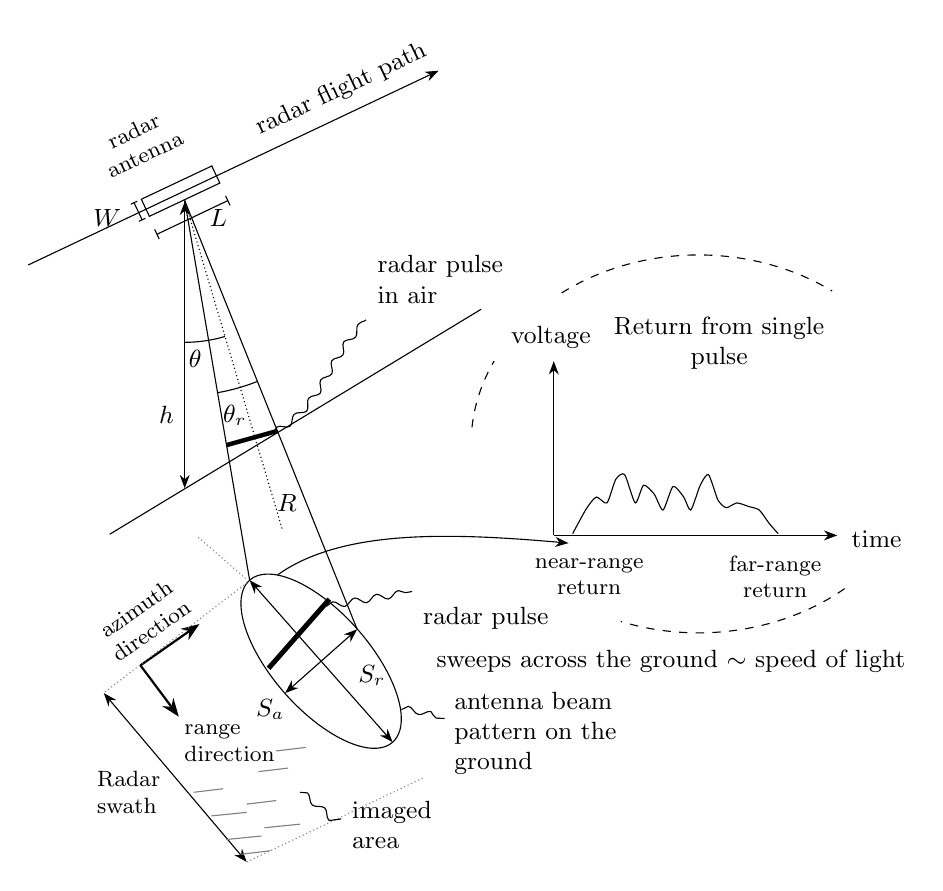
\begin{tikzpicture}[x=0.075mm, y=-0.075mm, >=Stealth, font=\small]
		% flight path and ground (nadir) line
		\draw[->] (290,397) -- (985,68);
		\node[rotate=25.3, anchor=south] at (835,132) {radar flight path};
		\draw (428,853) -- (1057,472);
		% antenna: center (548,272); u = (0.904,-0.427) along track, n = (0.427,0.904)
		\draw ($(548,272)+66*(-0.904,0.427)+16*(-0.427,-0.904)$) -- ($(548,272)+66*(0.904,-0.427)+16*(-0.427,-0.904)$)
			-- ($(548,272)+66*(0.904,-0.427)+16*(0.427,0.904)$) -- ($(548,272)+66*(-0.904,0.427)+16*(0.427,0.904)$) -- cycle;
		\node[rotate=25.3, anchor=south, align=center, font=\footnotesize] at (500,236) {radar\\antenna};
		% W marker (across the short side, left of the antenna)
		\draw ($(476,306)+16*(-0.427,-0.904)$) -- ($(476,306)+16*(0.427,0.904)$);
		\draw ($(476,306)+16*(-0.427,-0.904)+6*(-0.904,0.427)$) -- ($(476,306)+16*(-0.427,-0.904)+6*(0.904,-0.427)$);
		\draw ($(476,306)+16*(0.427,0.904)+6*(-0.904,0.427)$) -- ($(476,306)+16*(0.427,0.904)+6*(0.904,-0.427)$);
		\node[anchor=east] at (464,318) {$W$};
		% L marker (below the antenna)
		\draw (508,345) -- (628,288);
		\draw ($(508,345)+9*(-0.427,-0.904)$) -- ($(508,345)+9*(0.427,0.904)$);
		\draw ($(628,288)+9*(-0.427,-0.904)$) -- ($(628,288)+9*(0.427,0.904)$);
		\node at (612,318) {$L$};
		% altitude h
		\draw[<->] (555,290) -- (555,775);
		\node[anchor=east] at (553,650) {$h$};
		% beam edges and center line (footprint center at (786,1068))
		\draw[thin] (555,288) -- (665,931);
		\draw[thin] (555,288) -- (847,1014);
		\draw[densely dotted] (555,288) -- (720,844);
		% theta (look angle) and theta_r (range beamwidth)
		\draw (555,288) ++(90:240) arc[start angle=90, end angle=73.5, radius=240];
		\node at (573,556) {$\theta$};
		\draw (555,288) ++(80.3:330) arc[start angle=80.3, end angle=68.1, radius=330];
		\node at (640,652) {$\theta_r$};
		% radar pulse in air
		\draw[line width=1.6pt] (626,702) -- (712,678);
		\draw[decorate, decoration={snake, amplitude=1.2pt, segment length=8pt}] (704,682) to[out=30, in=220] (862,490);
		\node[anchor=south west, align=left] at (865,478) {radar pulse\\in air};
		\node at (728,800) {$R$};
		\begin{scope}[shift={(60,0)}]
		% footprint ellipse: center (726,1068) before the shift, semi-axes 183 and 82, major axis at 48.56 deg
		\draw plot[domain=0:360, samples=90, smooth cycle] ({726+183*cos(\x)*0.6617-82*sin(\x)*0.7497},{1068+183*cos(\x)*0.7497+82*sin(\x)*0.6617});
		\draw[<->] (605,931) -- (847,1205);
		\draw[<->] (665,1122) -- (787,1014);
		\node at (640,1150) {$S_a$};
		\node at (812,1092) {$S_r$};
		% radar pulse on the ground
		\draw[line width=1.8pt] (637,1080) -- (740,963);
		\draw[decorate, decoration={snake, amplitude=1.2pt, segment length=8pt}] (735,975) to[out=10, in=190] (880,950);
		\node[anchor=north west, align=left] at (882,960) {radar pulse};
		\node[anchor=west] at (905,1068) {sweeps across the ground ${\sim}$ speed of light};
		% antenna beam pattern on the ground
		\draw[decorate, decoration={snake, amplitude=1.2pt, segment length=8pt}] (862,1150) to[out=0, in=180] (935,1165);
		\node[anchor=west, align=left] at (935,1190) {antenna beam\\pattern on the\\ground};
		% curved arrow from the near edge of the footprint to the near-range return
		\draw[->] (652,922) .. controls (760,845) and (940,850) .. (1145,868);
		% azimuth and range directions
		\draw[->, thick] (420,1075) -- (520,1005);
		\draw[->, thick] (420,1075) -- (485,1162);
		\node[rotate=35, anchor=south, align=center, font=\footnotesize] at (455,1040) {azimuth\\direction};
		\node[anchor=north west, align=left, font=\footnotesize] at (478,1160) {range\\direction};
		% radar swath
		\draw[<->] (358,1122) -- (600,1408);
		\node[anchor=east, align=left, font=\footnotesize] at (470,1290) {Radar\\swath};
		% imaged area
		\draw[densely dotted, gray] (360,1120) -- (603,933);
		\draw[densely dotted, gray] (518,858) -- (598,928);
		\draw[densely dotted, gray] (600,1408) -- (900,1265);
		\foreach \y/\xa/\xb in {1290/510/560, 1330/540/600, 1370/565/625, 1310/600/650, 1350/630/690, 1395/590/640, 1255/620/670, 1220/650/700} {
			\draw[gray, thin] (\xa,\y) -- (\xb,\y-6);
		}
		\draw[decorate, decoration={snake, amplitude=1.2pt, segment length=8pt}] (690,1290) to[out=-30, in=180] (760,1335);
		\node[anchor=west, align=left] at (762,1345) {imaged\\area};
		\end{scope}
		% inset: return from a single pulse
		\draw[->] (1180,855) -- (1180,560);
		\draw[->] (1180,855) -- (1660,855);
		\node[anchor=south] at (1175,555) {voltage};
		\node[anchor=west] at (1668,862) {time};
		\node[align=center] at (1460,530) {Return from single\\pulse};
		\draw plot[smooth, tension=0.4] coordinates {(1212,852) (1235,810) (1252,790) (1270,800) (1285,760) (1300,752) (1318,800) (1332,770) (1350,785) (1365,812) (1382,772) (1400,790) (1412,812) (1428,770) (1442,752) (1458,795) (1472,808) (1490,800) (1510,806) (1528,812) (1545,835) (1560,852)};
		\node[align=center, font=\footnotesize] at (1240,925) {near-range\\return};
		\node[align=center, font=\footnotesize] at (1555,925) {far-range\\return};
		\draw[dashed] (1425,700) ++(185:385 and 320) arc[start angle=185, end angle=206, x radius=385, y radius=320];
		\draw[dashed] (1425,700) ++(233:385 and 320) arc[start angle=233, end angle=306, x radius=385, y radius=320];
		\draw[dashed] (1425,700) ++(50:385 and 320) arc[start angle=50, end angle=110, x radius=385, y radius=320];
	\end{tikzpicture}
	\caption{Imaging geometry of a side-looking radar: the antenna (width $W$, length $L$) at altitude $h$ illuminates an elliptical footprint $S_r \times S_a$ on the ground at range $R$ and look angle $\theta$; each pulse sweeps across the footprint, and the echo from a single pulse (inset) runs from the near-range to the far-range return (cf.\ van Zyl (2011), Fig.~1-2).}
	\label{f:geom}
\end{figure}
% NOTE: the caption is added.

\begin{itemize}
	% NOTE: added "(Figure~\ref{f:geom})".
	\item Pulses transmitted from radar as platform moves (Figure~\ref{f:geom})
	% NOTE: checked against van Zyl 2011, Eqs. 1.4-1 to 1.4-4 (pp. 11-12; his S, the swath, is S_r here; theta is the
	% look angle at the center of the swath; theta_r small). The underbrace "flat-Earth assumption" is handwritten.
	% The ~= signs are handwritten. theta_r, theta_a, S_r, S_a, W, L, h, theta are flagged in master table D156-D160.
	\item Each pulse illuminates an ellipse on the ground
	\begin{itemize}
		\item[--] defined in range:
		\begin{equation}
			\label{e:Sr}
			\theta_r \approx \frac{\lambda}{W} \qquad \text{and} \qquad \underbrace{S_r \approx \frac{h\theta_r}{\cos^2\theta}}_{\text{flat-Earth assumption}} = \frac{\lambda h}{W\cos^2\theta}
		\end{equation}
		\item[--] in azimuth:
		\begin{equation}
			\label{e:Sa}
			\theta_a \approx \frac{\lambda}{L} \qquad \text{and} \qquad S_a \approx R\theta_a \approx \frac{\lambda h}{L\cos\theta}
		\end{equation}
	\end{itemize}
	% NOTE: checked against van Zyl 2011, p. 12 (same example, x_a = 16 km); python3: 16.3 km. 23 cm is 1.30 GHz,
	% L-band (U&L 2014, Table 1-5, p. 18: 0.39-1.55 GHz).
	\item[] E.g.\ for a spacecraft: $h = 800$~km, $\lambda = 23$~cm (L-band), $L = 12$~m, $\theta = 20^\circ$ $\rightarrow$ $S_a = 16$~km
\end{itemize}

%%%%%%%%%%%%%%%%%%%%%%%%%%%%%%%%%%%%%
% ---- page L5 ----
% NOTE: subsection heading added.
\subsection{Azimuth resolution of a real-aperture radar}
\label{s:rar}

\begin{itemize}
	\item For a real-aperture radar, $S_a = X_a \equiv$ azimuth resolution
	\begin{itemize}
		% NOTE: handwritten "Resolution defines smallest object that can be uniquely detected"; corrected to "smallest
		% separation between two objects that can be uniquely detected", because resolution is "that separation between
		% the two closest features that can still be resolved in the final image" (van Zyl 2011, p. 6); an object smaller
		% than the resolution cell can still be detected if it is bright enough.
		\item[--] Resolution defines smallest separation between two objects that can be uniquely detected
		\item[--] Note example on previous page $\rightarrow$ $X_a = 16$~km is \underline{horrible} resolution
		% NOTE: handwritten "2 cm (X-band)"; corrected to "2 cm (Ku-band)": 2 cm is 15 GHz, above X-band (U&L 2014,
		% Table 1-5, p. 18: X = 5.75-10.9 GHz, i.e., 2.8-5.2 cm; K = 10.9-36 GHz, whose lower part, 10.9-22 GHz, is
		% commonly called Ku-band); van Zyl (2011, p. 12), the source of the example, gives only "2 cm". The value 2 cm
		% and the result are kept. Handwritten "X = 360 m" written X_a. Checked: python3 gives X_a = 355 m (van Zyl:
		% "about 360 m").
		\item[--] Even if we decrease $\lambda$ to 2~cm (Ku-band) and made $h = 200$~km (unreasonably low altitude for a satellite), $X_a = 360$~m, which is still pretty \underline{lousy} resolution for most science applications
		% NOTE: checked against van Zyl 2011, p. 12 and p. 13 ("Real aperture radars are therefore not commonly used for
		% remote sensing applications").
		\item[--] Poor resolution limits application of real-aperture radar for RS applications, though there are some notable exceptions $\rightarrow$ terrestrial radar
		% NOTE: "azimuth" is a caret insertion before "resolution" in the scan. Checked against van Zyl 2011, Eq. 1.5-7
		% (p. 15).
		\item[--] Synthetic aperture techniques will dramatically improve azimuth resolution, and will lead to azimuth resolution equal to half the length of the antenna!!! Will discuss how in a bit
	\end{itemize}
\end{itemize}

% NOTE: subsection heading added.
\subsection{Range resolution}
\label{s:range}

\begin{itemize}
	\item What is range resolution?
	\begin{itemize}
		% NOTE: added "(Figure~\ref{f:angles})".
		\item[--] First, distinguish slant range and ground range (Figure~\ref{f:angles})
	\end{itemize}
\end{itemize}

\begin{figure}[!htbp]
	\centering
	% Reproduces the handwritten sketch (page L5) element by element (cf. van Zyl 2011, Fig. 1-3, p. 5): the radar
	% (dot, upper left, labeled); a dashed horizontal line from the radar (no arrowhead) and a dashed vertical line
	% from the radar down to the ground (no arrowhead); the slant range (line from the radar to the target, arrowheads at
	% both ends, label along the line); the ground range (line from the foot of the vertical to the target, arrowheads
	% at both ends, label below); the depression angle (arc between the horizontal and the slant range) and the look
	% angle (arc between the vertical and the slant range), with labels; the target (dot, labeled); the local unit
	% normal (arrow up from the target, handwritten n-hat, written a-hat); the incidence angle (arc between the normal
	% and the slant range; handwritten theta, written theta_i) and the grazing angle (arc between the ground and the
	% slant range), with labels; and, beside the sketch, the note "theta != look angle on curved planet" (theta
	% written theta_i).
	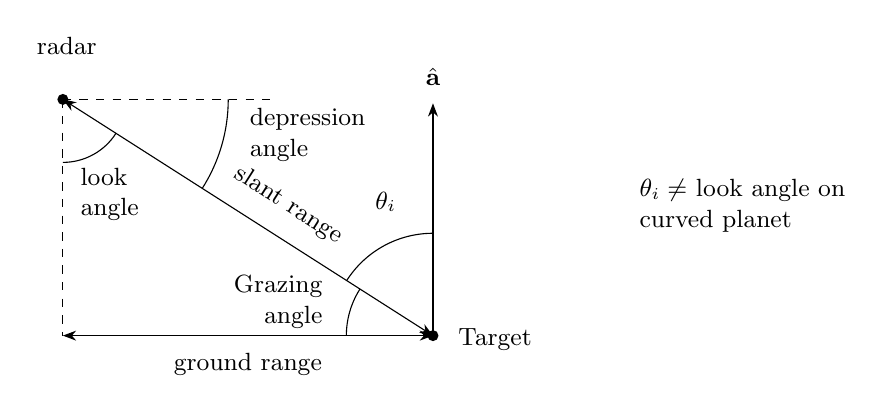
\begin{tikzpicture}[x=0.1mm, y=-0.1mm, >=Stealth, font=\small]
		\coordinate (Rd) at (180,115);
		\coordinate (Tg) at (650,415);
		\coordinate (F) at (180,415);
		\fill (Rd) circle (7);
		\node[anchor=south] at (185,70) {radar};
		\draw[dashed] (Rd) -- (450,115);
		\draw[dashed] (Rd) -- (F);
		\draw[<->] (Rd) -- (Tg);
		\draw[<->] (F) -- (Tg);
		\fill (Tg) circle (7);
		\node[anchor=west] at (670,420) {Target};
		\node[anchor=north] at (415,425) {ground range};
		\node[rotate=-32.55, anchor=south] at (452,272) {slant range};
		% depression angle (horizontal 0 deg to slant 32.55 deg, pixel frame) and look angle (slant 32.55 to vertical 90)
		\draw (Rd) ++(0:210) arc[start angle=0, end angle=32.55, radius=210];
		\node[anchor=west, align=left] at (405,160) {depression\\angle};
		\draw (Rd) ++(32.55:80) arc[start angle=32.55, end angle=90, radius=80];
		\node[anchor=north west, align=left] at (190,190) {look\\angle};
		% normal and angles at the target
		\draw[->] (Tg) -- (650,120);
		\node[anchor=south] at (650,110) {$\hat{\mathbf{a}}$};
		\draw (Tg) ++(-90:130) arc[start angle=-90, end angle=-147.45, radius=130];
		\node at (590,245) {$\theta_i$};
		\draw (Tg) ++(180:110) arc[start angle=180, end angle=212.55, radius=110];
		\node[anchor=east, align=right] at (522,372) {Grazing\\angle};
		\node[anchor=west, align=left] at (900,250) {$\theta_i \neq$ look angle on\\curved planet};
	\end{tikzpicture}
	\caption{Slant range, ground range and the angles that describe the imaging geometry (cf.\ van Zyl (2011), Fig.~1-3). Neglecting the curvature of the Earth, and for a surface without topography, the look angle equals the incidence angle $\theta_i$.}
	\label{f:angles}
\end{figure}
% NOTE: the caption is added; its second sentence is from van Zyl 2011, p. 5 ("When surface curvature effects are
% neglected, the look angle is equal to the incidence angle at the surface when the surface is flat").

\begin{itemize}
	\item[] \begin{itemize}
		% NOTE: checked against van Zyl 2011, pp. 4-5.
		\item slant range $\equiv$ distance from radar to scatterer (target)
		\item ground range $\equiv$ distance from nadir point to scatterer along a smooth (not necessarily flat) surface
	\end{itemize}
	\item[] \begin{itemize}
		% NOTE: checked against van Zyl 2011, Eq. 1.2-1 (p. 6).
		\item[--] Now consider two point targets separated by a \underline{slant} range distance $X_r$ $\Rightarrow$ echoes will be separated in time
		\begin{equation}
			\label{e:dt}
			\Delta t = \frac{2X_r}{c}
		\end{equation}
	\end{itemize}
\end{itemize}

% ---- page L6 ----
% NOTE: subsubsection heading added (the scan's "Range resolution (cont.)" is a continuation mark).
\subsubsection{Pulse length and resolution}

\begin{itemize}
	% NOTE: checked against van Zyl 2011, pp. 6-7 and Fig. 1-5.
	\item[--] Radars transmit pulses, i.e., short bursts of energy
	\item[--] For a pulse w/ constant frequency, two scatterers can be distinguished if the \underline{leading edge} of the pulse from 2\textsuperscript{nd} scatterer is received after the trailing edge of pulse from 1\textsuperscript{st} scatterer (Figure~\ref{f:pulses})
	% NOTE: added "(Figure~\ref{f:pulses})".
\end{itemize}

\begin{figure}[!htbp]
	\centering
	% Reproduces the two handwritten sketches (page L6) element by element (cf. van Zyl 2011, Fig. 1-5, p. 7): in each
	% panel, a voltage axis (arrowhead up) and a time axis t (arrowhead right); dimension lines with end bars (no
	% arrowheads) for Delta t and tau (handwritten bare tau, written tau_eff); scatterer dots below the time axis.
	% Top: two hatched boxes labeled "pulse", separated so that Delta t >= tau_eff; labels "scatterer 1", "scatterer 2";
	% note "Delta t >= tau_eff => scatterers are resolvable". Bottom: a hatched box labeled "pulse" and an overlapping
	% open box starting at Delta t < tau_eff (overlap hatched); Delta t and tau_eff dimension lines above, and a second
	% tau_eff from Delta t; two dots, the first with a short tick below it (unlabeled); note "Delta t < tau_eff =>
	% scatterers not (underlined) resolvable for monochrome pulse".
	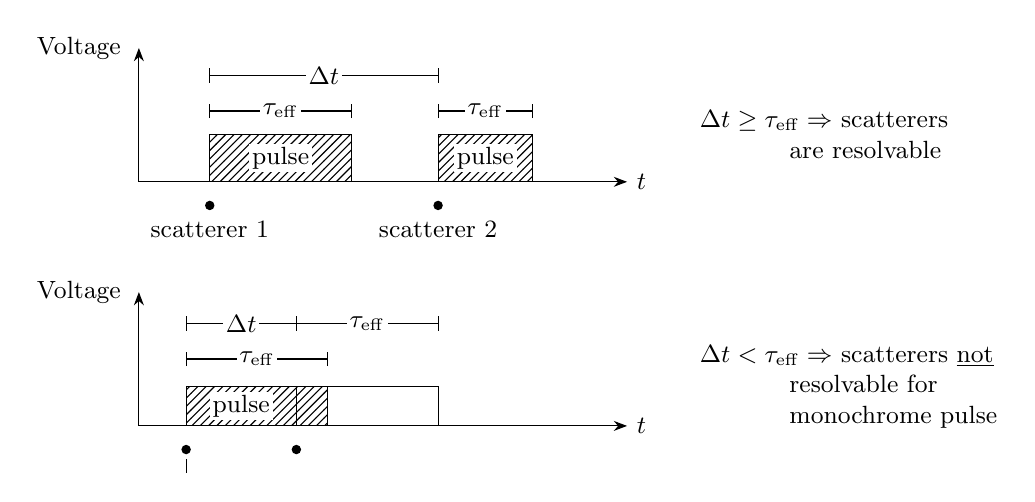
\begin{tikzpicture}[>=Stealth, font=\small]
		\def\dim#1#2#3#4{\draw (#1,#3) -- (#2,#3); \draw (#1,#3-0.09) -- (#1,#3+0.09); \draw (#2,#3-0.09) -- (#2,#3+0.09); \node[fill=white, inner sep=1pt] at ({(#1+#2)/2},#3) {#4};}
		% top panel
		\begin{scope}
			\draw[->] (0,0) -- (0,1.7) node[anchor=east, xshift=-3pt] {Voltage};
			\draw[->] (0,0) -- (6.2,0) node[anchor=west] {$t$};
			\draw[pattern=north east lines] (0.9,0) rectangle (2.7,0.6);
			\node[fill=white, inner sep=1pt] at (1.8,0.3) {pulse};
			\draw[pattern=north east lines] (3.8,0) rectangle (5.0,0.6);
			\node[fill=white, inner sep=1pt] at (4.4,0.3) {pulse};
			\dim{0.9}{2.7}{0.9}{$\teff$}
			\dim{3.8}{5.0}{0.9}{$\teff$}
			\dim{0.9}{3.8}{1.35}{$\Delta t$}
			\fill (0.9,-0.3) circle (0.06);
			\node[anchor=north] at (0.9,-0.38) {scatterer 1};
			\fill (3.8,-0.3) circle (0.06);
			\node[anchor=north] at (3.8,-0.38) {scatterer 2};
			\node[anchor=west, align=left] at (7.0,0.6) {$\Delta t \ge \teff \Rightarrow$ scatterers\\\hspace*{3.5em}are resolvable};
		\end{scope}
		% bottom panel
		\begin{scope}[yshift=-3.1cm]
			\draw[->] (0,0) -- (0,1.7) node[anchor=east, xshift=-3pt] {Voltage};
			\draw[->] (0,0) -- (6.2,0) node[anchor=west] {$t$};
			\draw (0.6,0) rectangle (2.4,0.5);
			\draw (2.0,0) rectangle (3.8,0.5);
			\fill[pattern=north east lines] (0.6,0) rectangle (2.4,0.5);
			\node[fill=white, inner sep=1pt] at (1.3,0.25) {pulse};
			\dim{0.6}{2.4}{0.85}{$\teff$}
			\dim{0.6}{2.0}{1.3}{$\Delta t$}
			\dim{2.0}{3.8}{1.3}{$\teff$}
			\fill (0.6,-0.3) circle (0.06);
			\draw (0.6,-0.42) -- (0.6,-0.6);
			\fill (2.0,-0.3) circle (0.06);
			\node[anchor=west, align=left] at (7.0,0.5) {$\Delta t < \teff \Rightarrow$ scatterers \underline{not}\\\hspace*{3.5em}resolvable for\\\hspace*{3.5em}monochrome pulse};
		\end{scope}
	\end{tikzpicture}
	\caption{Echoes from two point scatterers for a constant-frequency (monochromatic) pulse of length $\teff$: resolvable when their separation in time is $\Delta t \ge \teff$ (top), not resolvable when $\Delta t < \teff$ (bottom) (cf.\ van Zyl (2011), Fig.~1-5).}
	\label{f:pulses}
\end{figure}
% NOTE: the caption is added.

\begin{itemize}
	% NOTE (page L6): handwritten bare tau ("pulse length"; on page L8, "effective pulse duration tau = 1/B") written
	% tau_eff throughout, because bare tau is the Fresnel transmission coefficient (instructor decision D18; precedent
	% tau_opt, D137); flagged in master table D150. For the constant-frequency pulse considered here, the effective
	% pulse length equals the true pulse duration tau_p of page L8 (van Zyl 2011, p. 7: "the effective time length tau
	% of the pulse"; Eq. 1.2-5, tau = 1/B). Checked against van Zyl 2011, Eq. 1.2-2 (p. 7). Handwritten "seperable"
	% written "separable".
	\item[--] Thus, smallest separable $\Delta t = \teff$, where $\teff \equiv$ pulse length
	\begin{equation}
		\label{e:xr}
		\Rightarrow\quad \frac{2X_r}{c} = \Delta t = \teff \quad\Rightarrow\quad X_r = \frac{c\teff}{2}
	\end{equation}
	\item[--] What does this mean for ground range resolution?
	% NOTE (page L6): handwritten theta written theta_i (incidence angle; master table), as in the page L5 sketch.
	% van Zyl 2011 (p. 7) specifies that it is the local incidence angle (theta_i' in the master table, Lectures 7-8),
	% which is what the slope remark below refers to. Checked against van Zyl 2011, Eqs. 1.2-3 and 1.2-4 (p. 7).
	\item[--] Two point targets w/ ground range separation $X_g$
	\begin{equation}
		\label{e:dtg}
		\Delta t = \frac{2X_g\sin\theta_i}{c}
	\end{equation}
	% NOTE: the box and the arrow to it are handwritten. Scope (NOTE only): the statement is exact for the slant-range
	% resolution X_r (Eq. e:xr); X_g contains no range, but at fixed altitude theta_i grows across the swath with
	% ground range, so X_g decreases from near to far range (it is independent of distance only at fixed theta_i).
	\item[--] Based on argument above,
	\begin{equation}
		\label{e:xg}
		X_g = \frac{c\teff}{2\sin\theta_i} \quad \longrightarrow \quad \boxed{\text{No dependence on distance to target!!!}}
	\end{equation}
	% NOTE: checked against van Zyl 2011, p. 8 ("For slopes facing the radar, the ground range resolution will be
	% poorer than that for slopes facing away from the radar").
	\item[--] Note the dependence of ground range resolution on incidence angle $\Rightarrow$ for slopes facing radar, $\theta_i$ decreases $\Rightarrow$ $X_g$ increases (and vice versa)
	\begin{itemize}
		\item[$\bigstar$] ground range resolution varies dramatically in mountains
	\end{itemize}
\end{itemize}

% ---- page L7 ----
% NOTE: subsubsection heading added.
\subsubsection{Noise and the pulse length}

\begin{itemize}
	\item[--] It would appear at this point that improving resolution is a simple matter of reducing the pulse duration $\teff$
	\item[--] Why would we not want to do that?
	\item[--] A.\ Noise
	\begin{itemize}
		% NOTE: "Recall lecture on radiation" refers to Lectures 12-13 (Planck's law).
		\item Recall lecture on radiation: Planck's law tells us that any material w/ $T > 0$~K emits radiation at a range of frequencies
		% NOTE (page L7): handwritten reads "thermal noise power density P_N = K_B T Delta f/lambda^2" and "received power
		% density P_r"; corrected to "thermal noise power P_N = k_B T Delta f" and "received power P_r", because the SNR
		% is a ratio of powers: P_r is the received power in watts (Lecture 7, Eq. e:Pr there), and the thermal noise
		% power in a receiver of bandwidth Delta f is k_B T Delta f (van Zyl 2011, Eqs. 1.3-1 and 1.3-2, p. 10-11,
		% P_N = kTB, SNR = P_r/P_N; Lecture 13, Eq. e:Pbb there, P_bb = k_B T Delta f), whereas k_B T Delta f/lambda^2 is
		% a brightness in W m^-2 sr^-1 (Lecture 13, Eq. e:I there), so P_r/P_N would not be dimensionless. Handwritten
		% K_B written k_B (D14). T is the total equivalent noise temperature (van Zyl p. 11). P_N is flagged in master
		% table D162. (van Zyl, p. 11, gives k = 1.6e-23 W/K/Hz; the Boltzmann constant is 1.38e-23 J/K; book error,
		% not propagated.)
		\item Radars must operate at $T > 0$~K $\Rightarrow$ there will always be some thermal noise power
		\begin{equation}
			\label{e:PN}
			\PN = k_BT\Delta f
		\end{equation}
		\begin{itemize}
			\item[] $k_B \equiv$ Boltzmann's const
			% NOTE: checked against van Zyl 2011, p. 11 ("the noise bandwidth is usually larger than the transmit
			% bandwidth").
			\item[] $\Delta f \equiv$ bandwidth of instrument (not necessarily same as pulse bandwidth)
		\end{itemize}
		\item Signal to noise ratio is then simply received power $P_r$ divided by $\PN$
		\begin{equation}
			\label{e:SNR}
			\mathrm{SNR} = \frac{P_r}{\PN}
		\end{equation}
		% NOTE: checked against van Zyl 2011, p. 8. (With a receiver bandwidth matched to a constant-frequency pulse,
		% Delta f ~ 1/tau_eff, Eqs. e:PN and e:SNR give SNR ~ P_r tau_eff/(k_B T), the received energy per pulse
		% divided by k_B T; derivation, NOTE only.)
		\item To increase SNR, want to maximize energy in each pulse $\rightarrow$ can be done by increasing peak power or by using a longer pulse
		\item Peak power usually limited by power supply (esp.\ on satellites) $\Rightarrow$ increasing SNR depends on lengthening pulse duration
	\end{itemize}
	\item[--] There is a direct conflict between SNR and range resolution!
	\begin{itemize}
		\item longer pulse $=$ higher SNR (good), lower resolution (bad)
		\item shorter pulse $=$ lower SNR (bad), higher resolution (good)
	\end{itemize}
\end{itemize}

%%%%%%%%%%%%%%%%%%%%%%%%%%%%%%%%%%%%%
% ---- page L8 ----
% NOTE: subsection heading added.
\subsection{Frequency-modulated pulses (chirp)}
\label{s:chirp}

\begin{itemize}
	% NOTE: checked against van Zyl 2011, p. 8.
	\item[--] The solution to SNR--resolution conundrum is to abandon monochromatic pulses and to modulate the frequencies instead
	\item[--] `chirp' -- signal whose frequency changes in time
	% NOTE: checked against van Zyl 2011, Eqs. 1.2-6 and 1.2-7 (p. 8), which write f_0 in both terms of B. Here Delta f
	% is the frequency excursion of the chirp, not the instrument bandwidth Delta f of Eq. (e:PN) (flagged in master
	% table D151, with B and f_0). tau_p is kept as handwritten; tau (bare) written tau_eff (D150; see page L6).
	\item[--] Radar generally uses a linear chirp
	\begin{equation}
		\label{e:ft}
		\Rightarrow\quad f(t) = f_0 + \frac{B}{\tau_p}t \qquad \text{for } -\frac{\tau_p}{2} \le t \le \frac{\tau_p}{2}
	\end{equation}
	where
	\begin{itemize}
		\item[] $B = |(f + \Delta f) - f| = |\Delta f| \equiv$ pulse bandwidth
		\item[] $\tau_p \equiv$ true pulse duration (different from effective pulse duration $\teff = 1/B$)
	\end{itemize}
	% NOTE: checked against van Zyl 2011, Eq. 1.2-5 (p. 8) and p. 9.
	\item[--] Note that $B = 1/\teff$ is a property of radar instrument while $\tau_p$ is the true pulse duration
	\begin{itemize}
		% NOTE: from Eqs. (e:xr) and (e:xg) with tau_eff = 1/B: X_r = c/(2B), X_g = c/(2B sin theta_i).
		\item[$\bigstar$] Range resolution $X_r \sim X_g \sim \dfrac{1}{B}$
		\item[$\bigstar$] SNR scales w/ $\tau_p$
		% NOTE: handwritten "and short pulse duration tau_p (=> high SNR)"; corrected to "long", because SNR scales with
		% tau_p (two lines above; page L7) and van Zyl 2011 (p. 8): "a pulse with long duration (i.e., high energy) and
		% wide bandwidth (i.e., high range resolution) can be constructed."
		\item[$\bigstar$] Using frequency modulated (FM) pulses, possible to construct system and pulse w/ high bandwidth ($\Rightarrow$ fine resolution) and long pulse duration $\tau_p$ ($\Rightarrow$ high SNR)
	\end{itemize}
	% NOTE: checked against van Zyl 2011, Eq. 1.2-8 (p. 8), A(t) ~ cos[2 pi (f_0 t + B t^2/(2 tau_p))], with omega_0 =
	% 2 pi f_0; the phase is 2 pi times the integral of f(t) (Eq. e:ft) (python3/sympy: 2 pi f_0 t + pi B t^2/tau_p). A(t) is flagged in master table D153.
	\item[--] Signal amplitude of chirped signal
	\begin{equation}
		\label{e:At}
		A(t) \sim \cos\!\left(\omega_0t + \frac{\pi B}{\tau_p}t^2\right) \qquad \text{for } -\frac{\tau_p}{2} \le t \le \frac{\tau_p}{2}
	\end{equation}
	\item[--] Matched filtering allows for recovery of fine-resolution features from pulse train $\rightarrow$ range compression
\end{itemize}

% ---- page L9 ----
% NOTE: subsection heading from the handwritten bullet "Range compression" (page L9).
\subsection{Range compression}
\label{s:rc}

\begin{itemize}
	% NOTE: checked against van Zyl 2011, p. 9. The three-dot sign before "FM pulse" is read as "because" (low-confidence
	% reading; possibly "therefore"), which fits the sense of the sentence.
	\item[--] Echoes from different scatterers will overlap in time, but $\because$ FM pulse echoes will have different frequencies $\Rightarrow$ can be separated by appropriate filtering
	\item[--] Matched filters often used in radar processing
	\begin{itemize}
		\item Idea is simple: the signal received from a scatterer will be a scaled replica of the transmitted signal delayed by time $t = 2R/c$
		% NOTE: "convolve return signal w/ transmit signal" kept as handwritten (van Zyl 2011, p. 9, uses the same
		% wording); Eq. (e:Vo) below is the convolution of V_r with the time-reversed complex conjugate of A,
		% i.e., the matched filter.
		\item Therefore, simply convolve return signal w/ transmit signal
		% NOTE (page L9): handwritten A(t) = A_0 e^{j(omega(t) t + phi)}; corrected to A_0 e^{j(omega_0 t + pi B t^2/tau_p +
		% phi)}, the complex form of the chirp of Eq. (e:At): with omega(t) = 2 pi f(t) (Eq. e:ft), omega(t) t = omega_0 t +
		% 2 pi B t^2/tau_p, twice the quadratic phase of Eq. (e:At), whose derivative would give a sweep rate of 2B/tau_p;
		% the instantaneous frequency is the derivative of the phase divided by 2 pi (van Zyl 2011, Eq. 1.2-8 and p. 8).
		% A_0, phi, V_r, V_o, E_r, xi are flagged in master table D152-D155. V_o (van Zyl: V_o, "o" for output) is
		% handwritten V with a subscript read as o or 0 (low-confidence reading). A, V_r and V_o are complex-valued time
		% signals written without a tilde (see D153).
		\item To illustrate, suppose a transmit signal
		\begin{equation}
			\label{e:Acplx}
			A(t) = A_0\,e^{j(\omega_0t + \pi Bt^2/\tau_p + \phi)} \qquad \text{for } -\frac{\tau_p}{2} \le t \le \frac{\tau_p}{2}
		\end{equation}
		% NOTE: added (instructor decision on master table D153, 2026-09-30): the complex (analytic) signal carries no
		% tilde here, as in van Zyl; the physical signal is its real part, the chirp of Eq. (e:At).
		(the physical signal is the real part of $A(t)$, i.e., the chirp of Eq.~\eqref{e:At})
		and the received signal is
		\begin{equation}
			\label{e:Vr}
			V_r(t) = E_rA\!\left(t - \frac{2R}{c}\right)
		\end{equation}
		% NOTE (page L9): handwritten "= tau_p E_r e^{j(omega t - 2KR)} sin(...)/(...)"; corrected by adding the factor
		% |A_0|^2 (the product A^*(xi - t) V_r(xi) contains A_0^* A_0; phi cancels) and writing "~=", because the result
		% holds for a large time-bandwidth product B tau_p >> 1 near the peak, |t - 2R/c| << tau_p (van Zyl 2011,
		% Eq. 1.2-9, p. 9: "for large time-bandwidth products"). Exact result (derivation): tau_p |A_0|^2 E_r e^{j omega_0
		% (t - 2R/c)} sin[pi B u (1 - |u|/tau_p)]/(pi B u), u = t - 2R/c, |u| <= tau_p (python3,
		% B tau_p = 1000: the numerically integrated convolution matches this exact result to 7 significant figures
		% at u = 0, 1/(4B), 1/B, 3/B, and differs from the sinc form of Eq. (e:Vo) by at most 3e-3 of the peak). Handwritten omega written omega_0 (van Zyl: omega = 2 pi f_0) and K written k
		% (D14), k = 2 pi/lambda, so 2kR = 4 pi R/lambda (van Zyl's exp(-i 4 pi R/lambda)). The underbrace label is
		% handwritten.
		\item[] then the compressed radar signal is the convolution
		\begin{align}
			\Vo(t) &= \int_{-\infty}^{\infty}A^*(\xi - t)\,V_r(\xi)\,d\xi \nonumber\\
			&\approx \tau_p|A_0|^2E_r\,e^{j(\omega_0t - 2kR)}\,\underbrace{\frac{\sin\!\left(\pi B(t - 2R/c)\right)}{\pi B(t - 2R/c)}}_{\text{norm.\ sinc function}} \label{e:Vo}
		\end{align}
	\end{itemize}
	% NOTE: handwritten "a half power width of 1/B"; corrected to "approximately 1/B" (van Zyl 2011, p. 9: "This
	% compressed pulse has a half power width of approximately 1/B"): the full width at half power of sinc^2(Bu) is
	% 0.886/B (python3); the first nulls are at +-1/B.
	\item Peak of compressed pulse occurs at $t = \dfrac{2R}{c}$ and it has a half power width of approximately $\dfrac{1}{B}$, consistent w/ our previous observation that range resolution $\sim \dfrac{1}{B}$
\end{itemize}

%%%%%%%%%%%%%%%%%%%%%%%%%%%%%%%%%%%%%
% ---- page L10 ----
% NOTE: section heading from the handwritten underlined heading "Synthetic Aperture Radar (SAR)" (page L10).
\section{Synthetic aperture radar (SAR)}
\label{s:sar}

\begin{itemize}
	% NOTE: "imaging radar" is a caret insertion between "utilizes" and "data" in the scan. Checked against van Zyl
	% 2011, p. 13.
	\item `Synthetic aperture radar' utilizes imaging radar data collected from a moving platform and a special processing technique that stitches together many pulses to synthesize a much larger antenna (aperture)
	\item Key is to recognize that a target will be seen by the radar at different points in the radar footprint during different pulses $\Rightarrow$ slight differences in angles w.r.t.\ velocity vector $\Rightarrow$ Doppler shift
	\item Using Doppler effect, multiple targets can be separated in the azimuth direction $\Rightarrow$ greatly improving azimuth resolution for a given radar instrument
	% NOTE: checked against van Zyl 2011, p. 13 ("The range resolution and radar equation derived previously for a real
	% aperture radar are still valid here").
	\item Use of Doppler effect to compress signals in azimuth is the difference between SAR and real-aperture radar
	\begin{itemize}
		\item[$\hookrightarrow$] range resolution and compression discussed before are the same for SAR and real-aperture radars
	\end{itemize}
	% NOTE: the handwritten line "* - See movie of pulse radar - *" (an in-class instruction) is omitted.
	% NOTE: added "(Figure~\ref{f:sar})".
	\item So, SAR relies on Doppler effect and sensor motion (Figure~\ref{f:sar})
\end{itemize}

\begin{figure}[!htbp]
	\centering
	% Reproduces the handwritten sketch (page L10) element by element (cf. van Zyl 2011, Fig. 1-7, p. 14): the radar
	% flight path (line to the upper right, arrowhead at its end) and its label; the scatterer (dot) and its label; the
	% antenna beam when the scatterer enters the beam (wedge from a point on the flight path; its right edge ends at the
	% scatterer, its left edge runs down to the lower left) with the azimuth beamwidth theta_a (arc at the apex between
	% the two edges); the range at closest approach R_0 (line from the flight path to the scatterer, no arrowheads); the
	% antenna beam when the scatterer exits the beam (wedge from a later point on the flight path; its left edge ends
	% at the scatterer); labels for both beams; the nadir line (parallel to the flight path, drawn only outside the two
	% wedges, as in the scan) and its label.
	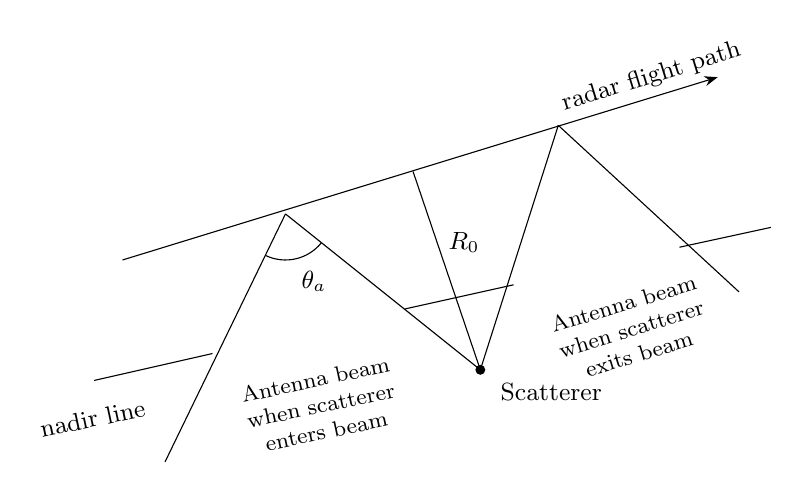
\begin{tikzpicture}[x=0.09mm, y=-0.09mm, >=Stealth, font=\small]
		\coordinate (P1) at (400,290);
		\coordinate (M) at (580,230);
		\coordinate (P2) at (785,165);
		\coordinate (S) at (675,510);
		\draw[->] (170,355) -- (1010,97);
		\node[rotate=17.1, anchor=south] at (925,125) {radar flight path};
		% beams
		\draw (P1) -- (230,640);
		\draw (P1) -- (S);
		\draw (P2) -- (S);
		\draw (P2) -- (1040,400);
		\draw (M) -- (S);
		\node at (652,330) {$R_0$};
		% theta_a at P1 between the left edge (toward (230,640)) and the right edge (toward S)
		\draw (P1) ++(115.9:65) arc[start angle=115.9, end angle=38.4, radius=65];
		\node at (440,385) {$\theta_a$};
		% nadir line, drawn outside the two wedges
		\draw (130,525) -- (297,487);
		\draw (569,424) -- (722,390);
		\draw (956,337) -- (1085,309);
		\node[anchor=east, rotate=12] at (215,560) {nadir line};
		\fill (S) circle (7);
		\node[anchor=north west] at (690,515) {Scatterer};
		\node[rotate=12, align=center, font=\footnotesize] at (450,560) {Antenna beam\\when scatterer\\enters beam};
		\node[rotate=17, align=center, font=\footnotesize] at (888,452) {Antenna beam\\when scatterer\\exits beam};
	\end{tikzpicture}
	\caption{The synthetic aperture: a scatterer at range of closest approach $R_0$ is observed for as long as it remains in the antenna beam of azimuth beamwidth $\theta_a$, from the pulse at which it enters the beam to the pulse at which it exits (cf.\ van Zyl (2011), Fig.~1-7).}
	\label{f:sar}
\end{figure}
% NOTE: the caption is added.

% ---- page L11 ----
% NOTE: subsection heading added (the scan's heading "Synthetic Aperture Radar (SAR) (cont.)" is a continuation
% mark).
\subsection{Doppler history of a point scatterer}
\label{s:doppler}

\begin{itemize}
	% NOTE (page L11): checked against van Zyl 2011, Eq. 1.5-1 (p. 14). The platform velocity is handwritten V or v
	% (case unclear); written v, as in van Zyl (V is the voltage V_r, V_o on page L9). s (slow time) and v are flagged
	% in master table D161; R_0 in D152.
	\item Distance between antenna and scatterer as a function of time $s$ (a.k.a.\ slow time)
	\begin{equation}
		\label{e:Rs}
		R(s) = \sqrt{R_0^2 + v^2s^2}
	\end{equation}
	\begin{itemize}
		\item[] $R_0 \equiv$ minimum distance from flight path to scatterer
		\item[] $v \equiv$ platform velocity
	\end{itemize}
	% NOTE: handwritten "R_0 ~= R_0 + v^2 s^2/(2 R_0)"; corrected to "R(s) ~=", because the left side is the range as a
	% function of slow time, expanded to first order in (vs/R_0)^2 (van Zyl 2011, Eq. 1.5-2, p. 14; python3/sympy series).
	\item Usually in RS, $vs \ll R_0$
	\begin{equation}
		\label{e:Rapprox}
		\Rightarrow\quad R(s) \approx R_0 + \frac{v^2}{2R_0}s^2
	\end{equation}
	% NOTE: checked against van Zyl 2011, Eq. 1.5-3 (p. 14); the phase is that of the second exponential in Eq. (e:Vo),
	% -2kR = -4 pi R/lambda.
	\item The phase after range compression (see expression on previous pages) is given as
	\begin{equation}
		\label{e:phis}
		\phi(s) = -\frac{4\pi R(s)}{\lambda} \approx -\frac{4\pi R_0}{\lambda} - \frac{2\pi v^2}{R_0\lambda}s^2
	\end{equation}
	% NOTE: checked against van Zyl 2011, Eq. 1.5-4 (p. 15).
	\item The instantaneous frequency is simply
	\begin{equation}
		\label{e:fs}
		f(s) = \frac{1}{2\pi}\frac{\partial\phi(s)}{\partial s} = -\frac{2v^2}{R_0\lambda}s \qquad (s = 0 \text{ when } R = R_0)
	\end{equation}
	% NOTE: the handwritten arrow from "this" to Eq. (e:fs) is written as the equation reference.
	\item Note that this, Eq.~\eqref{e:fs}, is expression of linear chirp, just like we saw for FM pulse
	\item To find Doppler bandwidth $\rightarrow$ maximum time we can use for signal integration $\rightarrow$ amount of time scatterer is in antenna footprint
\end{itemize}

% NOTE: subsection heading added.
\subsection{SAR azimuth resolution}
\label{s:sarres}

\begin{itemize}
	% NOTE: checked against van Zyl 2011, Eq. 1.5-5 (p. 15). The handwritten time symbol is read s_tot (slow time;
	% van Zyl: s_tot); the s is written like a capital S (low-confidence reading).
	\item As discussed before, for an antenna w/ along-track length $L$,
	\begin{equation}
		\label{e:stot}
		\theta_a = \frac{\lambda}{L} \quad\Rightarrow\quad \stot = \frac{\lambda R_0}{Lv}
	\end{equation}
	% NOTE: checked against van Zyl 2011, Eq. 1.5-6 (p. 15). |f(s_tot)| equals the total sweep f(-s_tot/2) -
	% f(s_tot/2) because f(s) is linear in s (Eq. e:fs); python3: with the exact R(s) of Eq. (e:Rs), B_D = 2v/L to
	% 1e-4 for R_0 = 100-1500 km. The handwritten subscript of B_D (D for Doppler, as in van Zyl) could also be read as
	% 0 (low-confidence reading). B_D is flagged in master table D151.
	\item Doppler bandwidth
	\begin{equation}
		\label{e:BD}
		\BD = |f(\stot)| = \frac{2v}{L}
	\end{equation}
	% NOTE: checked against van Zyl 2011, Eq. 1.5-7 (p. 15). The box is handwritten. Handwritten "match filter
	% approach" written "matched filter approach".
	\item Using matched filter approach (as with range compression), the compressed signal will have a duration $1/\BD$
	\begin{equation}
		\label{e:XSAR}
		\Rightarrow\quad \text{Azimuth resolution} \quad \boxed{\XSAR = \frac{v}{\BD} = \frac{L}{2}}
	\end{equation}
	\hspace*{\fill}$\rightarrow$ Amazing! only a function of length of physical antenna!!!
\end{itemize}

% ---- page L12 ----
\begin{itemize}
	% NOTE (page L12): the real-aperture resolution is Eq. (e:Sa), X_a = S_a ~= R lambda/L (van Zyl 2011, Eq. 1.4-4).
	\item SAR azimuth resolution
	\begin{equation}
		\label{e:compare}
		\XSAR = \frac{L}{2} \qquad \rightarrow \text{compare w/} \quad \XRAR = \frac{R\lambda}{L}
	\end{equation}
	\begin{itemize}
		% NOTE: checked against van Zyl 2011, p. 15 ("The smaller the physical antenna is, the larger its footprint. This
		% allows a longer observation time ... a larger Doppler bandwidth and, hence, a finer surface resolution");
		% B_D = 2v/L, Eq. (e:BD).
		\item[--] Smaller antenna $=$ finer resolution? Yes because smaller antenna result in broader footprints $\Rightarrow$ longer $\stot$ (time in beam) $\Rightarrow$ higher Doppler bandwidth
		% NOTE (page L12): handwritten "longer range gives broader footprint => higher Doppler bandwidth that cancels range
		% effect on resolution"; corrected to "=> longer s_tot (longer synthetic aperture) that cancels ...", because the
		% Doppler bandwidth B_D = 2v/L (Eq. e:BD) does not depend on range: s_tot grows as R_0 (Eq. e:stot) while the
		% Doppler rate 2v^2/(R_0 lambda) (Eq. e:fs) falls as 1/R_0. What grows with range is the synthetic aperture,
		% v s_tot = lambda R_0/L, whose angular resolution lambda/(2 v s_tot) = L/(2 R_0) cancels the factor R_0
		% (derivation; python3: B_D = 1400 Hz and X_a = 5.0 m for R_0 = 100-1500 km with v = 7 km/s, L = 10 m). (van Zyl
		% 2011, p. 15, also writes "larger Doppler bandwidth" here, which contradicts his Eq. 1.5-6; book error, not
		% propagated.)
		\item[--] No range dependence on azimuth resolution because longer range gives broader footprint $\Rightarrow$ longer $\stot$ (longer synthetic aperture) that cancels range effect on resolution
	\end{itemize}
	% NOTE: checked against van Zyl 2011, Eq. 1.5-8 (p. 16), PRF >= 2(B_D/2) = 2v/L (the Doppler frequency runs from
	% -B_D/2 to +B_D/2), and p. 16 ("at least one sample (i.e., one pulse) should be taken every time the sensor moves
	% by half an antenna length"). Handwritten "repitition" written "repetition".
	\item Since radar is pulsed, it's necessary to ensure pulse repetition frequency (PRF) sufficient to sample Doppler
	\begin{equation}
		\label{e:PRF}
		\Rightarrow\quad \mathrm{PRF} \ge \BD = \frac{2v}{L}
	\end{equation}
	\begin{itemize}
		\item[$\Rightarrow$] one sample should be taken when the antenna has moved at most $\dfrac{L}{2}$
	\end{itemize}
	% NOTE: handwritten "ambigaities" written "ambiguities".
	\item Next time, image artifacts, ambiguities and noise, then intro to InSAR
\end{itemize}

%%%%%%%%%%%%%%%%%%%%%%%%%%%%%%%%%%%%%
% Symbols follow the master table in ../variables_master.tex; see it for flagged dual usages.
\clearpage
\section*{Variables}

Units are SI; ``arb.'' marks signals in arbitrary units. Values are given for universal constants and for the examples in the notes.

{\small
\renewcommand{\arraystretch}{1.2}
\begin{longtable}{>{$}l<{$} >{\raggedright\arraybackslash}p{0.38\textwidth} >{\raggedright\arraybackslash}p{0.13\textwidth} >{\raggedright\arraybackslash}p{0.22\textwidth}}
\hline
\textrm{Symbol} & Description & Units & Value \\
\hline
\endfirsthead
\hline
\textrm{Symbol} & Description & Units & Value \\
\hline
\endhead
\hline
\endfoot
\multicolumn{4}{l}{\emph{Constants}} \\*
c & speed of light in a vacuum & m/s & $2.998\times10^{8}$ \\
k_B & Boltzmann constant & J/K & $1.381\times10^{-23}$ \\
j & imaginary unit & -- & $\sqrt{-1}$ \\
\multicolumn{4}{l}{\emph{Imaging geometry}} \\*
R & range (slant range) from the antenna to a target & m & $\frac12u_pt$ \\
t & time (round-trip travel time; time within a pulse) & s & -- \\
u_p & propagation (phase) velocity & m/s & $\approx c$ in air \\
\lambda & radar wavelength & m & 23~cm (L-band), 2~cm (Ku-band) in the examples \\
W, L & width and (along-track) length of the antenna & m & $L = 12$~m in the example \\
h & altitude of the radar above the surface & m & 800~km, 200~km in the examples \\
\theta & look angle (from the vertical to the beam center) & rad & $20^\circ$ in the example \\
\theta_r, \theta_a & beamwidths in range and azimuth & rad & $\lambda/W$, $\lambda/L$ \\
S_r, S_a & range and azimuth extents of the footprint on the ground & m & $\lambda h/(W\cos^2\theta)$, $\lambda h/(L\cos\theta)$ \\
\theta_i & incidence angle (from the local normal) & rad & $=\theta$ (flat Earth, no topography) \\
\hat{\mathbf{a}} & unit normal to the surface & dimensionless & -- \\
\multicolumn{4}{l}{\emph{Resolution}} \\*
X_a & azimuth resolution (real aperture: $S_a$) & m & 16~km, 360~m in the examples \\
X_a^\mathrm{RAR}, X_a^\mathrm{SAR} & azimuth resolution of a real- and a synthetic-aperture radar & m & $R\lambda/L$; $L/2$ \\
X_r, X_g & slant-range and ground-range resolutions (separations) & m & $c\teff/2$; $c\teff/(2\sin\theta_i)$ \\
\Delta t & separation in time of two echoes & s & -- \\
\teff & effective pulse length (duration) & s & $1/B$ \\
\tau_p & true pulse duration & s & -- \\
\multicolumn{4}{l}{\emph{Noise}} \\*
T & (total equivalent noise) temperature & K & -- \\
\Delta f & bandwidth of the instrument (L8: frequency excursion of the chirp, $|\Delta f| = B$) & Hz & -- \\
\PN & thermal noise power & W & $k_BT\Delta f$ \\
P_r & received power & W & -- \\
\mathrm{SNR} & signal-to-noise ratio & dimensionless & $P_r/\PN$ \\
\multicolumn{4}{l}{\emph{Chirp and range compression}} \\*
f, f(t) & frequency; instantaneous frequency of the chirp & Hz & $f_0 + Bt/\tau_p$ \\
f_0, \omega_0 & center (carrier) frequency and angular frequency & Hz; rad/s & $\omega_0 = 2\pi f_0$ \\
B & pulse (chirp) bandwidth & Hz & $1/\teff$ \\
A(t) & transmitted (chirp) signal & arb. & -- \\
A_0, \phi & amplitude and phase constant of $A(t)$ & arb.; rad & -- \\
V_r(t) & received signal & arb. & $E_rA(t - 2R/c)$ \\
\Vo(t) & compressed (matched-filter output) signal & arb. & -- \\
E_r & field received from a point scatterer (scale factor of the replica) & arb. & -- \\
\xi & integration variable (time) & s & -- \\
k & wavenumber, $2\pi/\lambda$ & rad/m & -- \\
\multicolumn{4}{l}{\emph{Synthetic aperture}} \\*
s & slow time (along the flight path) & s & 0 at closest approach \\
R(s), R_0 & range to the scatterer; range at closest approach & m & $\sqrt{R_0^2 + v^2s^2}$ \\
v & platform velocity & m/s & -- \\
\phi(s) & phase after range compression & rad & $-4\pi R(s)/\lambda$ \\
f(s) & instantaneous (Doppler) frequency & Hz & $-2v^2s/(R_0\lambda)$ \\
\stot & time the scatterer is in the beam & s & $\lambda R_0/(Lv)$ \\
\BD & Doppler bandwidth & Hz & $2v/L$ \\
\mathrm{PRF} & pulse repetition frequency & Hz & $\ge 2v/L$ \\
\end{longtable}
}

\end{document}
